\documentclass[11pt]{article}
\usepackage{../../latex/preamble}

\newcommand{\abs}[1]{|#1|}
\begin{document}
  % make title page
\begin{titlepage}
  \newcommand{\HRule}{\rule{\linewidth}{0.5mm}}
  \center
  \textsc{\LARGE Universitetet i Oslo}\\[1.5cm] % Name of your university/college
  \textsc{\Large }\\[0.5cm] % Major heading such as course name
  \textsc{\large FYS3150}\\[0.5cm] % Minor heading such as course title
  \HRule \\[0.4cm]
  { \huge \bfseries Ising-model blabla}\\[0.4cm]
  \HRule \\[1.5cm]
  \Large \emph{Skrevet av:}\\
  Lyder \textsc{Rumohr Blingsmo} og Bendik \textsc{Samseth}\\[3cm]
  {\large \today}\\[3cm]
  \vfill
\end{titlepage}

\begin{abstract}
I denne rapporten skal vi se på Ising-modellen i to dimensjoner. Det vil si
et rutenett av $n \times n $ partikler, der alle partiklene enten har
spinn opp, $\uparrow$ eller spinn ned, $\downarrow$. Spesielt ser vi
på de termodynamiske egenskapene til et slikt system. Vi bruker
Metropolis-algoritmen med 'periodic boundary conditions'. Alt materiale 
som refereres er tilgjengelig på~\cite{github-repo}. 
\end{abstract}

\section{Innledning}
\label{sec:innledning}
Ising-modellen er et system av $n \times n$ partikler ordnet i et rutenett. 
Hver partikkel kan være i én av to tilstander, enten spinn opp, $\uparrow$,
eller spinn ned, $\downarrow$. Energien er: 

\begin{equation}
  E=-J\sum_{<kl>}^{N}s_ks_l\label{eq:energi}
\end{equation}
med  $s_k=\pm 1$, $N$ er antall partikler.
$J$ er en konstant som beskriver styrken på interaksjonen mellom
nabopartikler. Symbolet $<kl>$ betyr at vi summerer over bare de
nærmeste naboene. Vi antar også  ferromagnetisme, dvs.  $J> 0$. Vi bruker også
periodiske randbetingelser. Det betyr at partiklene langs randa 'ser' 
partiklene langs motsatte rand. For eksempel 'ser' en partikkel i posisjon
(N,N) i rutenettet, både partikkelen i posisjon (1,N) og (N,1), og interakterer
med disse som om de skulle vært naboer. Vi bruker de termodynamiske størrelsene:

\begin{align}
Z &= \sum_i e^{-\beta E(i)} = \sum_E \Omega(E) e^{-\beta E}\label{eq:partisjons-funk} \\
C_V &= \frac{ 1 }{ k_B T^2} \left( \mean{E^2}-\mean{E}^2 \right)\label{eq:spesifikk-varmekapasitet} \\
\mathcal{M} &= \sum_i s_i\label{eq:magnetisering} \\
\chi &= \frac{ 1 }{ k_BT } \left( \mean{\mathcal{M}^2} - \mean{\mathcal{M}}^2 \right)\label{eq:susceptibilitet}.
\end{align}

Her er $\beta = 1/k_BT$, $Z$ partisjonsfunksjonen, $C_v$ er den spesifikke varmekapasiteten,
$\mathcal{M}$ er magnetiseringen og $\chi$ er susceptibiliteten. $E$, $T$ og $k_B$ er henholdsvis 
energien, temperaturen og boltzmannkonstanten. Disse størrelsene skal vi regne ut for flere forskjellige
størrelser på rutenettet og for mange forskjellige temperaturer.

\section{Implementering og testing}

Vi har tatt utgangspunkt i eksempelprogrammet \texttt{MPIising.cpp}
som finnes kursets Github-side~\cite{compphys-github}. Versjonen brukt
i denne rapporten er tilgjengelig på Github~\cite{github-repo} under samme navn. Kjernen av
programmet er Metropolisalgoritmen, som i vårt tilfelle går som følger: 

\begin{enumerate}
\item Initialiser en starttilstand med energi $E_0$, dvs. bestemmer retningen på
  alle spinn i systemet. Vi velger alle til å peke ned.
\item Velg en tilfeldig spinn og snu den.\label{steg2}
\item Beregn endringen i energi, $\Delta E = E_1-E_0$, dette fører til.\label{steg3} 
\item Dersom $\Delta E \leq 0$ godtar vi spinnendringen i håp om at vi
  er nærmere den minste mulige verdien av $E$. Gå til punkt (\ref{steg7}).
\item Dersom $\Delta E > 0 $, beregn Boltzmannsannsynligheten $w =
  e^{-\beta\Delta E}$. 
\item Sammenlikn $w$ med et tilfeldig tall $0\leq r\leq 1$ \label{steg6}
\begin{enumerate}
  \item Hvis $r\leq w$, godta spinnendringen
  \item ellers, behold den originale spinntilstanden.
\end{enumerate}
\item Oppdater relevante forventningsverdier og gjenta prosessen.\label{steg7}
  $N^2$ ganger, der $N^2$ er antall spinn.\footnote{Egentlig bare $N^2-1$ ganger fordi vi nå har gjort en
  allerede.}
\item Gjenta så steg (\ref{steg2})-(\ref{steg7}) mange ganger, der hver gjennomgang teller som
  én Monte Carlo-syklus.
\end{enumerate}

I steg (\ref{steg3}) beregner vi energiendringen. Når vi kun endrer på
én spinn om gangen er det kun 5 mulige verdier for $\Delta E$ for en
gitt verdi av $T$~\cite[s. 436]{Lecture-notes}. Derfor velger vi å
regne ut disse på forhånd og heller slå opp riktig verdi ved
behov. Dette gjør vi for å spare oss for mange gjentatte kall på en
eksponensialfunksjon. Vi regner med alle de termodynamiske \ref{eq:partisjons-funk} - \ref{eq:susceptibilitet}
 i enhetsløse størrelser. Tar som inputparametre størrelsen på rutenettet, antall Monte Carlo-sykluser,
inititiell temperatur, sluttemperatur, temperatursteg og en parameter som bestemmer om den initielle
spinkonfigurasjonen er tilfeldig eller ordnet.

\subsection{Test med $2 \times 2$-tilfellet}
For å få en intuisjon om hvordan et slikt system fungerer ser vi først på 
$2 \times 2$-tilfellet. Vi sammenligner programmet vårt med den 
eksakte løsningen i dette tilfellet. Vi ser for oss et rutenett av spinn
\begin{align*}
s_1 & s_2 \\
s_3 & s_4  
\end{align*}

Vi får da energien

\begin{align*}
E &= -J ( s_1s_2 + s_1s_3 + s_2s_1 + s_2s_4 \\
&  \hspace{1.1cm}+ s_3s_1 + s_3s_4 + s_4s_ + s_4s_3) \\ 
&= - J  ( 2s_1s_2 + 2s_1s_3 + 2s_2s_1 + 2s_2s_4 ) 
\end{align*}

Bruker vi spinn-konfigurasjonen
\begin{align*}
\uparrow & \uparrow \\
\uparrow & \uparrow
\end{align*}

Får vi energien 
\begin{align*}
E = - J  ( 2s_1s_2 + 2s_1s_3 + 2s_2s_1 + 2s_2s_4 ) = -J ( 8 \cdot 1 \cdot 1) = -8J  
\end{align*}
Gjør tilsvarende for alle mulige spinn-konfigurasjoner får vi tabell \ref{tab:spinn-energi-deg}:


\begin{table}[ht]
\centering
\caption{Tabell over energiene og degenerasjonene til de ulike
  spinn-konfigurasjonene til et $2\times 2$-rutenett av spinn.}
\label{tab:spinn-energi-deg}
\vspace{0.5cm}
% BEGIN RECEIVE ORGTBL spinnEnergi
\begin{tabular}{cccc}
Antall spinn opp & Degenerasjon & Energi & Magnetisering \\
\hline
4 & 1 & -8J & 4 \\
3 & 4 & 0 & 2 \\
2 & 4 & 0 & 0 \\
2 & 2 & 8J & 0 \\
1 & 4 & 0 & -2 \\
0 & 1 & -8J & -4 \\
\hline
\end{tabular}
% END RECEIVE ORGTBL spinnEnergi
\begin{comment}
#+ORGTBL: SEND spinnEnergi orgtbl-to-latex :splice nil :skip 0
| Antall spinn opp | Degenerasjon | Energi | Magnetisering |
|------------------+--------------+--------+---------------|
|                4 |            1 | -8J    |             4 |
|                3 |            4 | 0      |             2 |
|                2 |            4 | 0      |             0 |
|                2 |            2 | 8J     |             0 |
|                1 |            4 | 0      |            -2 |
|                0 |            1 | -8J    |            -4 |
|------------------+--------------+--------+---------------|
\end{comment}
\end{table}

Vi ser av tabell \ref{tab:spinn-energi-deg} at energien kan ha tre
mulige verdier, $E = -8J,0,8J$. Da er partisjonsfunksjonen gitt ved
likning (\ref{eq:partisjons-funk}) (bruker også degenerasjonsgradene
oppgitt i tabellen):
\begin{align}
  Z = \sum_E \Omega(E)e^{-\beta E} = 2e^{-\beta \cdot 8J} + 2e^{\beta
  \cdot 8J} + 12\label{eq:partisjons-funk-2x2}
\end{align}
Med partisjonsfunksjonen i boks kan vi finne alle forventningsverdier.

\begin{align}
\begin{split}
  \mean{E} &= \frac{ 1 }{ Z }\sum_E \Omega(E) E e^{-E\beta}\\
           &= 8J \frac{ e^{-8J\beta}  - e^{8J\beta}}{ e^{-8J\beta}
             + e^{8J\beta} + 6}\label{eq:mean-E-2x2}
\end{split}\\[0.5cm]
\begin{split}
  \mean{E^2} &= \frac{ 1 }{ Z }\sum_E E^2\Omega(E)e^{-E\beta}\\
  &= 64J^2 \frac{ e^{8J\beta} + e^{-8J\beta} }{ e^{-8J\beta} +
    e^{8J\beta} + 6 }\label{eq:mean-E2-2x2}
\end{split}\\[0.5cm]
  C_V &= \frac{ 1}{k_BT^2} \left( \mean{E^2} - \mean{E}^2 \right)\label{eq:mean-C-2x2}\\[0.5cm]
\begin{split}
  \mean{|\mathcal{M}|} &= \frac{ 1 }{ Z }\sum_i |\mathcal{M}_i| e^{-E_i\beta}\\
  &= \frac{ 4e^{8J\beta} + 8  }{ e^{-8J\beta} + e^{8J\beta} + 6 }.\label{eq:mean-abs-M-2x2}
\end{split}\\[0.5cm]
\mean{\mathcal{M}} &= 0\label{eq:mean-M-2x2}\\[0.5cm]
\begin{split}
  \mean{\mathcal{M}^2} &= \frac{ 1 }{ Z } \sum_i \mathcal{M}^2
  e^{-E_i\beta}\\
  &= 16 \frac{ e^{8J\beta} + 1 }{ e^{8J\beta} + e^{-8J\beta}+6 }\label{eq:mean-M2-2x2}
\end{split}\\[0.5cm]
\mean{\chi} &= \frac{ 1 }{ k_B T} \left(
              \mean{\mathcal{M}^2}-\mean{\mathcal{M}}^2
              \right)\label{eq:mean-chi-2x2}\\[0.5cm]
\mean{\chi}_\text{abs} &= \frac{ 1 }{ k_B T} \left( \mean{\mathcal{M}^2}-\mean{\mathcal{|M|}}^2 \right)\label{eq:mean-chi-2x2-abs}
\end{align}

Vi kan nå bruke disse formlene til å teste programmet. Vi velger å se
på $T=1$. Tabell \ref{tab:2x2-eksakt-num} viser både eksakte og
numeriske resultater. Etter litt testing kom vi frem til at ca. $10^6$
Monte Carlo-sykluser gir god overensstemmelse.


\begin{table}
\centering
\caption{Tabell over eksakte og numeriske resultater for $2\times
  2$-tilfellet for $T=1$. Vi har brukt $10^6$ Monte Carlo-sykluser. Merk at
alle tall er normalisert for antall spinn.}
\label{tab:2x2-eksakt-num}
\vspace{0.5cm}
\begin{tabular}{l|ccccc}
 & $\mean{E}$ & $\mean{ \abs{\mathcal{M} } }$ & $C_V$ & $\chi$ & $\chi_\text{abs}$ \\
\hline
Eksakt & -1.9959821 & 0.99866073 & 0.032082332 & 3.9933038 & 0.0040107395 \\
Numerisk & -1.9960480 & 0.99869100 & 0.031585527 & 3.9933824 & 0.0038971461 
\end{tabular}

\end{table}




\section{Resultater}

Vi begynner med å se på hvor lang tid systemet bruker på å stabilisere seg. I dette tilfellet
anser vi antall Monte Carlo-sykluser som et mål på tiden. For lave temperaturer ($T = 1$) ser vi at det
ordnede systemet begynner stabilt, som vil si i at det begynner i grunntilstanden, tilstanden med lavest energi. For lave temperaturer er det lite energi i systemet, og grunntilstanden er mest sannsynlig. Det uordnede
systemet bruker litt tid på å stabilisere seg, men vi ser fra \ref{fig:configurations} at også her går
antall konfigurasjoner mot 0 etter omtrent $3 \cdot 10^4$ sykluser. Det vil si at $w$ alltid er større $0\leq r\leq 1$ i steg \label{steg6} i Metropolis-algoritmen, og ingen spin-endringer blir gjort. Også systemet med høyere
temperatur ($T=2.4$) bruker cirka $3 \cdot 10^4$ sykluser på å stabilisere seg.

Ser vi derimot på antall konfigurasjoner i \ref{fig:configurations} ser vi at systemet med høy temperatur
har mange flere tilgjengelige tilstander enn det med lav temperatur. Det høres fornuftig ut, siden det har mer
'tilgjengelig' energi.

\begin{figure}[ht]

  \centering
  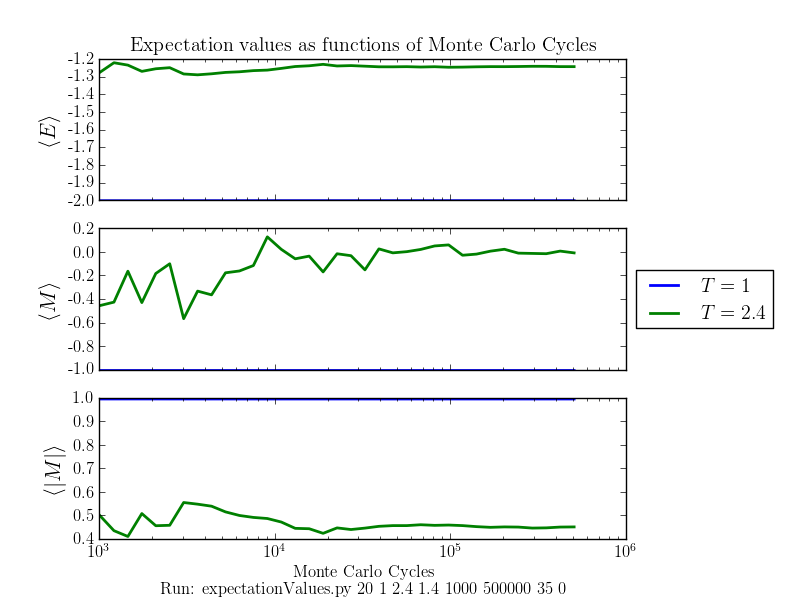
\includegraphics[scale=0.7]{../fig/E_M_Mabs.png}
  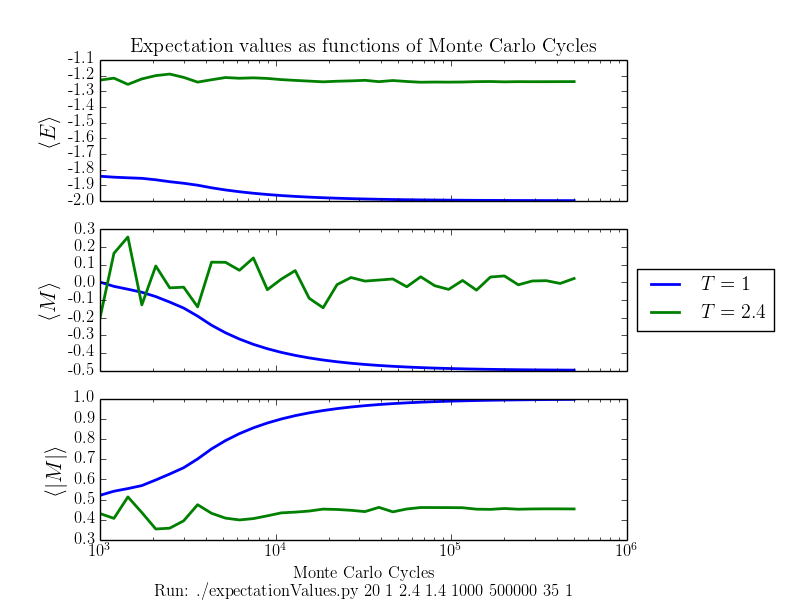
\includegraphics[scale=0.7]{../fig/E_M_Mabs_random.png}
  \caption{Plot av forventningsverdien til energi,
    magnetisering og absoluttverdien til magnetiseringa som funksjon av antall Monte Carlo-sykluser. 
    Øverst har vi det ordnede tilfellet der alle spins begynner med å peke ned. Det andre tilfellet er 
    med en tilfeldig startkonfigurasjon.}
\label{fig:forventningsverdi}
\end{figure}


\begin{figure}[ht]
  \centering
  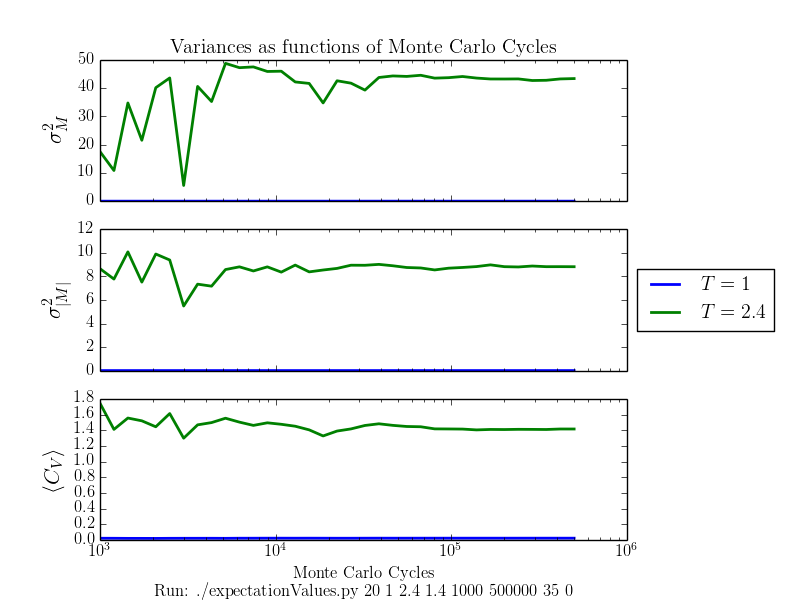
\includegraphics[scale=0.7]{../fig/variances.png}
  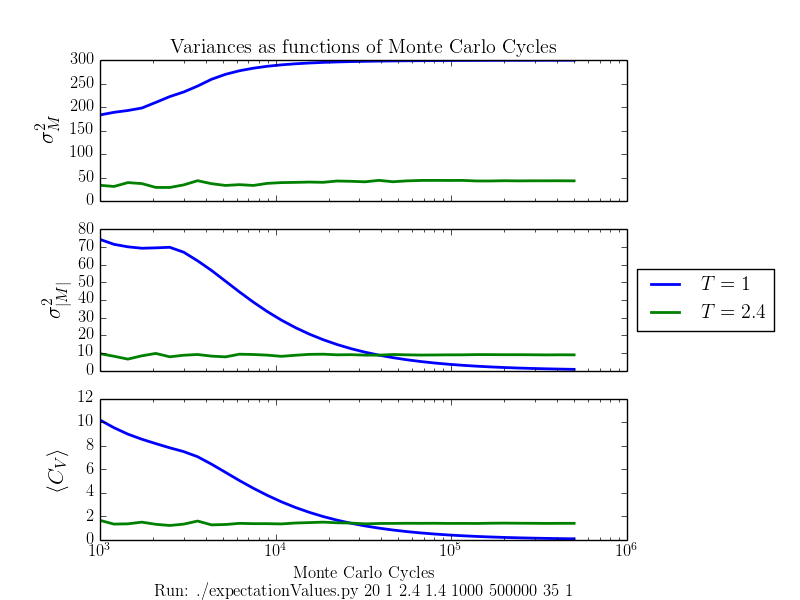
\includegraphics[scale=0.7]{../fig/variances_random.png}
  \caption{\label{fig:varianser} Plot av variansen til energien og magnetiseringa som
funksjon av antall Monte Carlo-sykluser. Variansen regner vi både med å bruke $\chi$ og $|\chi|$. Øverst
er det ordnete tilfellet, nederst det uordnede.}
\end{figure}


\begin{figure}[ht]
  \centering
  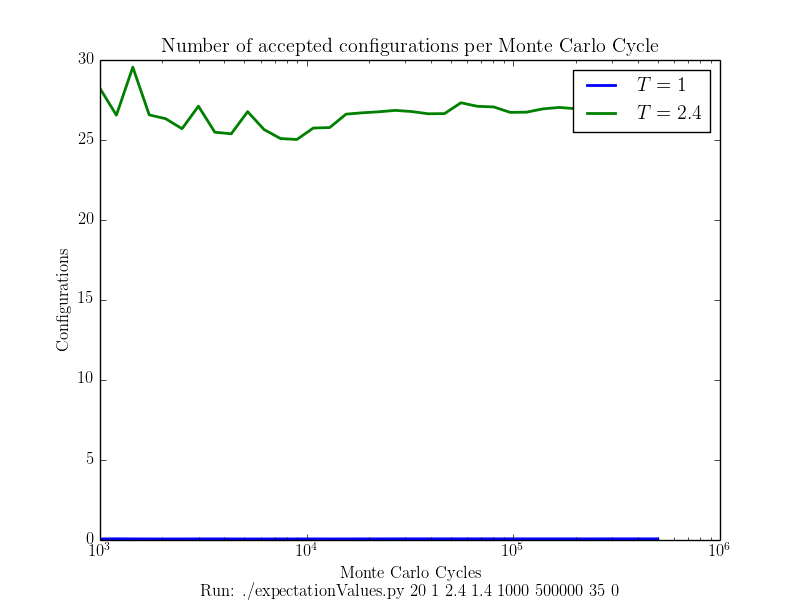
\includegraphics[scale=0.7]{../fig/configurations.png}
  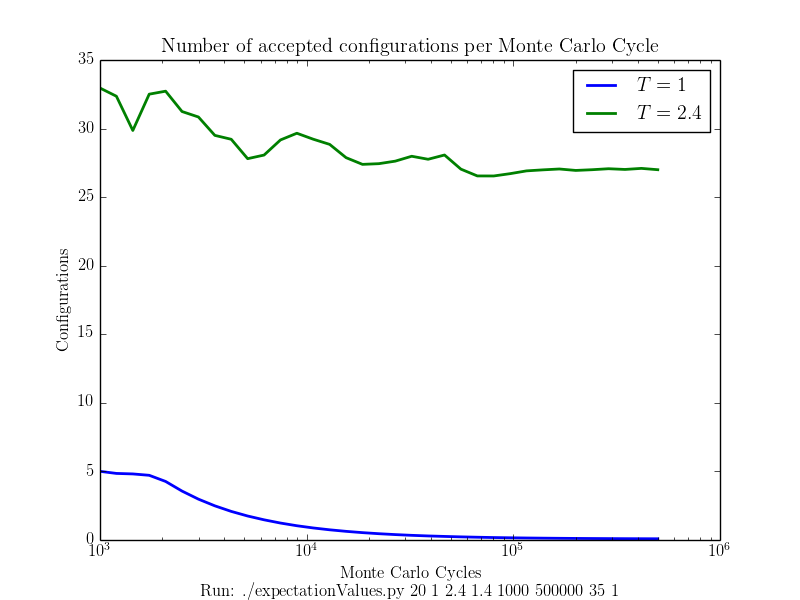
\includegraphics[scale=0.7]{../fig/configurations_random.png}

  \caption{\label{fig:configurations} Et plot av antall configurations
normalisert mot antall Monte Carlo-sykluser. Øverst er det ordnete tilfellet, nederst det uordnede.}
\end{figure}





\section{Konklusjon}

\clearpage
\printbibliography
\end{document}
%%% Local Variables:
%%% mode: latex
%%% TeX-master: t
%%% End:
